\documentclass{article}
\usepackage{graphicx}
\usepackage{float}
\usepackage{titlesec}
\usepackage{datetime}
\usepackage{geometry}
\usepackage{minted}
\usepackage{xcolor}
\usepackage{listings}
\usepackage{caption}
\usepackage{gensymb}
\usepackage[document]{ragged2e}
\usepackage[hidelinks]{hyperref}
\usepackage{booktabs}
\usepackage{placeins}

\geometry{
 a4paper,
 left=25mm,
 top=25mm,
 }
\newdateformat{daymonthyear}{\THEDAY .\THEMONTH .\THEYEAR}
\title{
  \centering
  
\includegraphics[width=\textwidth]{src/images/logo_PWr_kolor_poziom.png}\\
  \fontsize{28pt}{30pt}\selectfont Sprawozdanie 4\\
  \fontsize{14pt}{30pt}\selectfont Ćwiczenie 4.Systemy nawigacji satelitarnej(GPS)}
\author{Krzysztof Zalewa}
\date{\daymonthyear\today}

\renewcommand*\contentsname{Spis treści}
\renewcommand{\listingscaption}{Fragment kodu}
\begin{document}
  \maketitle
  \pagebreak
  \tableofcontents
  \pagebreak
  \section{Wstęp teoretyczny}
    \subsection{Systemy nawigacji satelitarnej}
    \subsubsection{Budowa i zasada działania systemu GPS}
    GPS składa się z konstelacji satelit umieszczonych na orbitach obecnie jest to aktywnych satelit i 3 zapasowe.
    GPS to system stadiometryczny co oznacza że pozycja wyznaczana jest na podstawie czasu propagacji sygnału z 
    satelit. Satelita wysyła sygnał z pewną częstoliwością, gdy sygnał ten dociera do odbiornika czas jest mierzony 
    i w połączeniu z czasem propagacji do innych widocznych satelit wyliczana jest lokalizacja(Rys1.)
    \begin{figure}[ht]
      \centering
      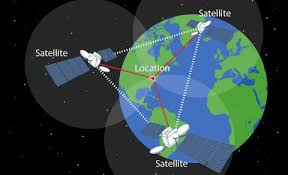
\includegraphics[width=\textwidth]{src/images/GPS.jpg}
      \caption{Schemat działania systemów stadiometrycznych}
      \label{fig:gps}
    \end{figure}
    \subsubsection{GLONASS [RF]}
    \sloppy
    To Rosyjski system nawigacji satelitarnej. Tak jak pozostałe systemy składa się z kosmicznego, kontroli i 
    użytkownika.Segment kosmiczny to 24 satelity umieszczone na 3 orbitach (po 8 na każdej). Satelity mają kąt 
    inklinacji równy 64,8\degree co pozwala na całkowite pokrycie kuli ziemskiej. Segmnet kontroli to główna stacja 
    kontrolna i kilka pomniejszych umieszconych w Europie,Rosji i Brazylii. Przez długi czas odbiorniki GLONASS 
    używane były w sprzęcie wojskowym, obecnie jednak są one dostępne dla użytkowników cywilnych.
    \subsubsection{Galileo [EU]}
    \sloppy
    To Europejski system nawigacji satelitarnej. Tak jak pozostałe systemy składa się z trzech segmentów kosmicznego, 
    kontroli i użytkownika. Segment kosmiczny to obecnie 24 satelit (z 30 planowanych) na trzech orbitach. Satelity 
    mają kąt inklinacji równy 56\degree. Co daje dobry sygnał głównie do serokości nawet 75\degree N (Najwyżej 
    położony punkt w europie).Segment kontroli znajduje się głównie w państwach europejskich. Segment użytkownika to 
    od samego początku (rok 2016) segment gospodarczy. 
    \subsubsection{BeiDou [Chiny]}
    \sloppy
    To Chiński system nawigacji satelitarnej. Obecna wersja (BeiDou-3) ma zasięg na całą kulę ziemską. Podbnie jak 
    pozostałe systemy składa się z trzech segmentów kosmicznego,kontroli i użytkownika. Segment kosmiczny to 24 
    satelity umieszczone na 3 orbitach. Segment kontroli znajduję się w chinach. A segent użytkownika to głównie 
    urządzenia militarne i komercjalne.
    \subsection{Struktura zdań NMEA}
    \raggedright
    Protokół opublikowany przez National Marine Electronics Association służy do komunikacji między morskimi 
    urządzeniami.Przykładowe zdanie NMEA: \linebreak
    \textbf{\$GPGGA,170834,N,41224.55000,08150.8500,W,1,05,1.5,280.2,M,-34.0,M,,,*75}
    \begin{table}[ht]
      \centering
      \begin{tabular}{p{7cm} p{3cm} p{4cm}}
        \toprule
        nazwa & przykładowa wartość &	opis \\
        \midrule
        Początek sekwencji& \$ &	początek sekwencji\\
        identyfikator nadawcy &	GP &	GPS\\
        rodzaj sekwencji &	GGA &	Global Positioning System Fix Data\\
        czas informacji &	170834 &	17:08:34 UTC\\
        szerokość geograficzna &	4124.5500, N &	41° 24,5500' N (41° 24' 33" N)\\
        długośc geograficzna &	08150.8500, W &	81° 50,8500' W (81° 50' 51" W)\\
        jakość pozycji &	1 &	jakość ustalonej pozycji (0 - nieważna, 1 - GPS, 2- DGPS...)\\
        liczba satelitów &	05 &	5 widocznych satelitów\\
        Horizontal Dilution of Precision (HDOP) &	1.5 &	dokładność pozycji (horyzontalna) = 1,5\\
        wysokość &	280.2, M & 280,2 ponad średni poziom morza\\
        wysokość geoidy ponad elipsoidę WGS84 &	-34.0, M & -34,0 metry\\
        czas od aktualizacji danych DGPS & pusta & brak\\
        identyfikator stacji nadającej poprawki różnicowe DGPS & pusta & brak\\
        suma kontrolna & *75 & używana do kontroli poprawności sentencji \\
        \bottomrule
      \end{tabular}
      \caption{Odczyt przykładowego zdania NMEA}
      \label{tab:nmea}
    \end{table}
    \FloatBarrier
  \raggedright
  \section{Zadanie laboratoryjne}
    \subsection{Treść zadania}
    W ramach zadania laboratoryjnego należało napisać program który będzie obsługiwał transmisję z urządzenia GPS.
    Program ten miał być w stanie rozkodować otrzymane zdania NMEA i zlokalizować na mapie punkt w którym znajduje 
    się urządzenie.
    \subsection{Opis działania programu}
    Po włączeniu program iteruje po wszystkich aktywnych portach COM. Do każdego portu wysyłane jest 20 pytań by 
    sprawdzić czy podpięte urządzenie to GPS. Jeżeli w odpowiedzi program dostanie conajmniej jedno poprawne 
    zdanie NMEA przechodzi on do głównej części zadanie. Co 200ms program pobiera zdanie NMEA i sprawdza jego 
    poprawność. Jeżeli zdanie jest poprawne to koordynaty wypisywane są w konsoli a na mapie pojawia się pinezka
    w odpowiednim miejscu. 
    \subsection{Kod programu}
        \begin{frame}
            \scriptsize
            \inputminted[
                style={vs},
                breaklines,
                breakanywhere, 
                linenos, 
                tabsize=4 
            ]{python}{Lab4.py}
            \vspace{1em}
            \captionsetup{justification=centering}
            \captionof{listing}{Kodu programu}
            \label{lst:code}
        \end{frame}      
  \section{Wnioski}
  Program udało się ukończyć na zajęciach i działał poprawnie. Na mapie pinezka pojawiała się w okolicach budynków
  C1,C2 i C3(W którym znajdowało się urządzenie).
  \section{Źródła}
  \begin{itemize}
    
    \item \url{https://gisplay.pl/nawigacja-satelitarna/glonass.html}
    \item \url{https://www.esa.int/Applications/Satellite_navigation/Galileo/What_is_Galileo}
    \item \url{https://defence-industry-space.ec.europa.eu/eu-space/galileo-satellite-navigation_en}
    \item \url{https://www.seinxon.com/en-eu/blogs/blog-posts/how-does-a-gps-tracker-work}
    \item \url{https://www.geotab.com/blog/what-is-gps/}
  \end{itemize}
\end{document}